\section{Comportamento}
Per comporamento del sito si intende il suo funzionamento dinamico, quindi
lato server, gestito dai file PHP, e lato client, gestito dal JavaScript.

\subsection{Javascript}
Per il comportamento di determinate pagine del sito, lato client, è stato utilizzato uno script in JavaScript che comprende diverse funzioni, le quali servono principalmente per il controllo dell’input nei form e nella barra di ricerca. È stato scelto di limitare al massimo l’utilizzo di queste funzionalità, in quanto non si possono fare assunzioni sulla disponibilità di tale tecnologia per tutta l’utenza del sito.\\
Inoltre, il sito è completamente fruibile nel caso JavaScript venga disabilitato,
in quanto è stata fornita un’alternativa lato server tramite PHP. Di seguito forniamo una breve descrizione del funzionamento degli script inseriti.

\subsubsection{Funzionalità}
Abbiamo usato un solo file per contenere tutte le funzionalità da noi implementate. Di seguito, la lista delle funzioni:
\begin{itemize}
	\item \textbf{load():} questa funzione viene chiamata quando tutto il contenuto della pagina è stato caricato. Quello che fa è assegnare un evento di \textit{click} al pulsante \textit{burger-menu} e al pulsante \textit{close}.\\
	Abbiamo scelto \textit{click} al posto di \textit{touch} perché il \textit{click} gestisce entrambi gli eventi. L'unica cosa negativa è che quando un utente usa le dita per cliccare il pulsante, l'evento non gestisce nel miglior modo l'area in cui l'utente clicca, siccome viene visto come un puntatore mouse e non come un dito. Per ovviare a questo problema abbiamo usato pulsanti un po' più grandi rispetto alla dimensione consigliata. Questo permette all'utente di non avere problemi nel tap sugli elementi.\\
	Il pulsante \textit{burger-menu} è situato nel top-right della pagina, mentre il \textit{close} sempre top-right ma all'interno del contenuto del menu che compare al di sotto dell'header;
	\item \textbf{scroll():} anche questa funzione viene chiamata alla fine del caricamento della pagina. Viene usata per far comparire un pulsante di aiuto alla navigazione, il quale permette di tornare ad inizio pagina quando un utente si trova al di sotto di una certa soglia di scrolling. Inoltre viene usata anche per il pulsante "torna all'articolo". Quando l'utente arriva a fine pagina, questo pulsante viene spostato leggermente più in alto per evitare che vada sopra al footer. Il suo posizionamento rispetto alla pagina è bottom-left. Grazie a questo pulsante non dovrà scrollare fino ad inizio pagina e quindi perdere tempo per tornare al contenuto da lui interessato. Il posizionamento del pulsante è bottom-right rispetto allo schermo per evitare che ingombri il contenuto della pagina e compare solo quando un utente scrolla.
	\item \textbf{plusClick():} questa funzione viene chiamata quando si clicca il pulsante + della pagina "Nuova Pagina". Serve per aggiungere delle pagine correlate alla pagina che l'utente sta creando. Ad ogni click, si aggiunge un menu a tendina contenente la lista di pagine del sito, in modo tale che l'utente selezioni la pagina correlata.
	\begin{figure}[H]
		\begin{center}
			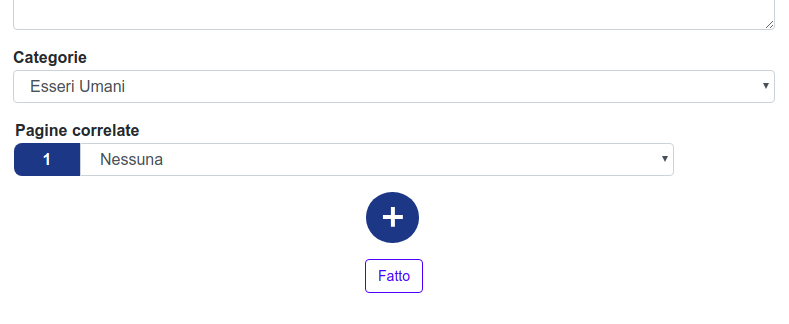
\includegraphics[width=10cm]{img/plusButton.jpg}
			\caption{Aggiunta pagine correlate}
		\end{center}
	\end{figure}
	\item \textbf{showAlert():} questa funzione viene chiamata quando un utente sta compilando un form e cambia focus di input. La funzione ha lo scopo di controllare se ciò che ha digitato l'utente sia corretto rispetto a ciò che vuole l'input. Se non è corretto, viene creato un "commento" al di sotto quell'input di colore rosso.
	\begin{figure}[htbp]
		\begin{center}
			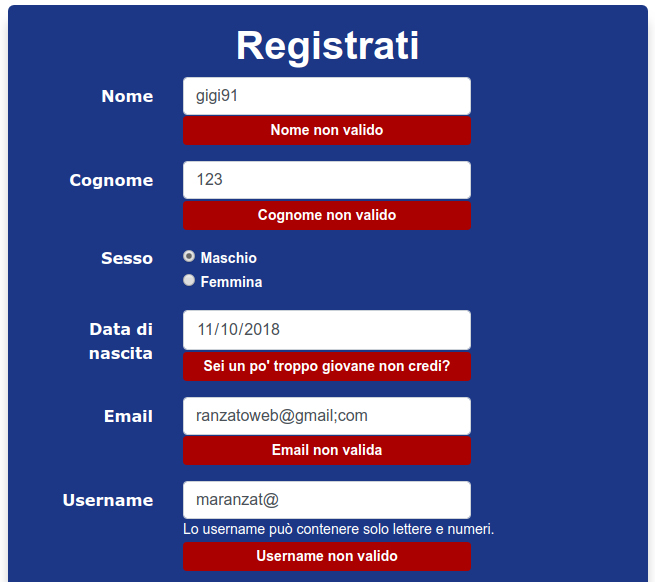
\includegraphics[width=10cm]{img/error.jpg}
			\caption{Errore di input}
		\end{center}
	\end{figure}
	\item \textbf{checkText():} questa funzione viene usata per controllare se il testo inserito dall'utente è corretto. Ritorna true se lo è, false se non lo è, e in questo caso, attraverso la chiamata alla funzione \textit{showAlert()} mostra l'errore di input all'utente. La funzione \textit{checkText()} viene usata per controllare i campi nome, cognome, email, username, password e conferma password;
	\item \textbf{checkEmail():} questa funzione viene usata allo stesso modo di \textit{checkText()} ma per il campo input email;
	\item \textbf{isPasswordEqual():} questa funzione viene usata allo stesso modo di \textit{checkText()} ma confronta il campo input password con conferma password;
	\item \textbf{AlertFileSize():} questa funzione controlla che l'immagine caricata dall'utente nella pagina "Nuova pagina" o "Modifica pagina", non sia troppo grande. Se lo è, il pulsante di submit viene disabilitato attraverso la funzione \textit{disableElement()};
	\item \textbf{disableElement():} questa funzione serve per disabilitare il pulsante di submit quando il form in "Nuova pagina" e "Modifica pagina" ha dei campi che non sono validi;
	\item \textbf{invalidBirthDay():} questa funzione viene usata per controllare se la data di nascita dell'utente è corretta, ovvero fa dei controlli per verificare l'età e, se è troppo piccolo, troppo vecchio oppure non viene inserita una data, non valida.
	
\end{itemize}
\pagebreak
\subsection{PHP}
Il comportamento del sito dal lato server è gestito da file PHP, i quali sostituiscono il JavaScript nel caso sia disabilitato, interagiscono con il database, forniscono sessioni di utilizzo per utenti loggati e caratterizzano il comportamento generale delle pagine.\\
Il codice PHP è stato suddiviso in diversi file, uno per ogni classe. Inoltre è stato creato un file che contiene un insieme di funzioni di supporto.

\subsubsection{Classi}
\paragraph{Gerarchia User} Abbiamo definito una classe che rappresenta un utente generico il quale ha una dipendenza verso la classe \textit{DatabaseConnection}. Le sottoclassi di User sono \textit{RegisteredUser} che rappresenta un semplice utente che si è registrato il quale ha una sottoclasse \textit{Admin} che specializza un utente registrato in un utente amministratore e \textit{UnregisteredUser} che rappresenta un utente non registrato. La responsabilità principale di questa gerarchia di classi è lo svolgimento delle query al database e il controllo di eventuali errori di connessione o di interazione con esso. Semanticamente, un utente effettua una connessione col database e ha la possibilità di interrogarlo o di interagirci. L'ereditarietà è stata utilizzata per gestire gli accessi e comprendere i privilegi in possesso all'utente definendo per ogni tipo le interazioni disponibili con la base di dati.

\subparagraph{User} 
La classe \textit{User} effettua la connessione al database tramite il costruttore ed espone i metodi per il reperimento delle informazioni.\\
I metodi più importanti sono:
\begin{itemize}
	\item \textbf{\texttt{searchArticle()}}: permette la ricerca per sottostringa, categoria, sottocategoria, tipo di pagina (pendenti o pubblicate) e autore;
	\item \textbf{\texttt{getArticleComment()}}: permette il reperimento dei commenti a un determinato articolo;
	\item \textbf{\texttt{getArticleInfo()}}: permette il reperimento delle informazioni di un determinato articolo dato il suo codice identificativo;
	\item \textbf{\texttt{getPathArticle()}}: permette il reperimento della categorie e della sottocategoria di un articolo.
\end{itemize}

\subparagraph{UnregisteredUser} 
La classe \textit{UnregisteredUser} espone la funzionalità di registrazione tramite il metodo \texttt{subscribe()}.

\subparagraph{RegisteredUser} 
La classe \textit{RegisteredUser} aggiunge alle funzionalità del supertipo quelle di modifica della base di dati.\\
I metodi principali sono:
\begin{itemize}
	\item \texttt{insertArticle()}: permette di inserire un nuovo articolo alla piattaforma, tale articolo sarà inserito come pendente;
	\item \texttt{modifyArticle()}: permette di inserire una modifica dell'articolo alla piattaforma;
	\item \texttt{deleteArticle()}: permette l'eliminazione di un articolo pubblicato;
	\item \texttt{declinePendant()}: permette la possibilità di eliminare una propria pagina pendente o una propria modifica in attesa di approvazione;
	\item \texttt{insertComment()}: permette di inserire un commento a un articolo.
\end{itemize}

\subparagraph{Admin}
La classe \textit{Admin} aggiunge la possibilità di approvare un articolo (\texttt{approveArticle()}) e di eliminare un utente \texttt{deleteUser()}.\\
Infine, sovrascrive il metodo \texttt{declinePendant()} di \textit{RegisteredUser}, permettendo di eliminare una qualsiasi pagina pendente o un qualsiasi modifica.

\begin{figure}[H]
	\begin{center}
		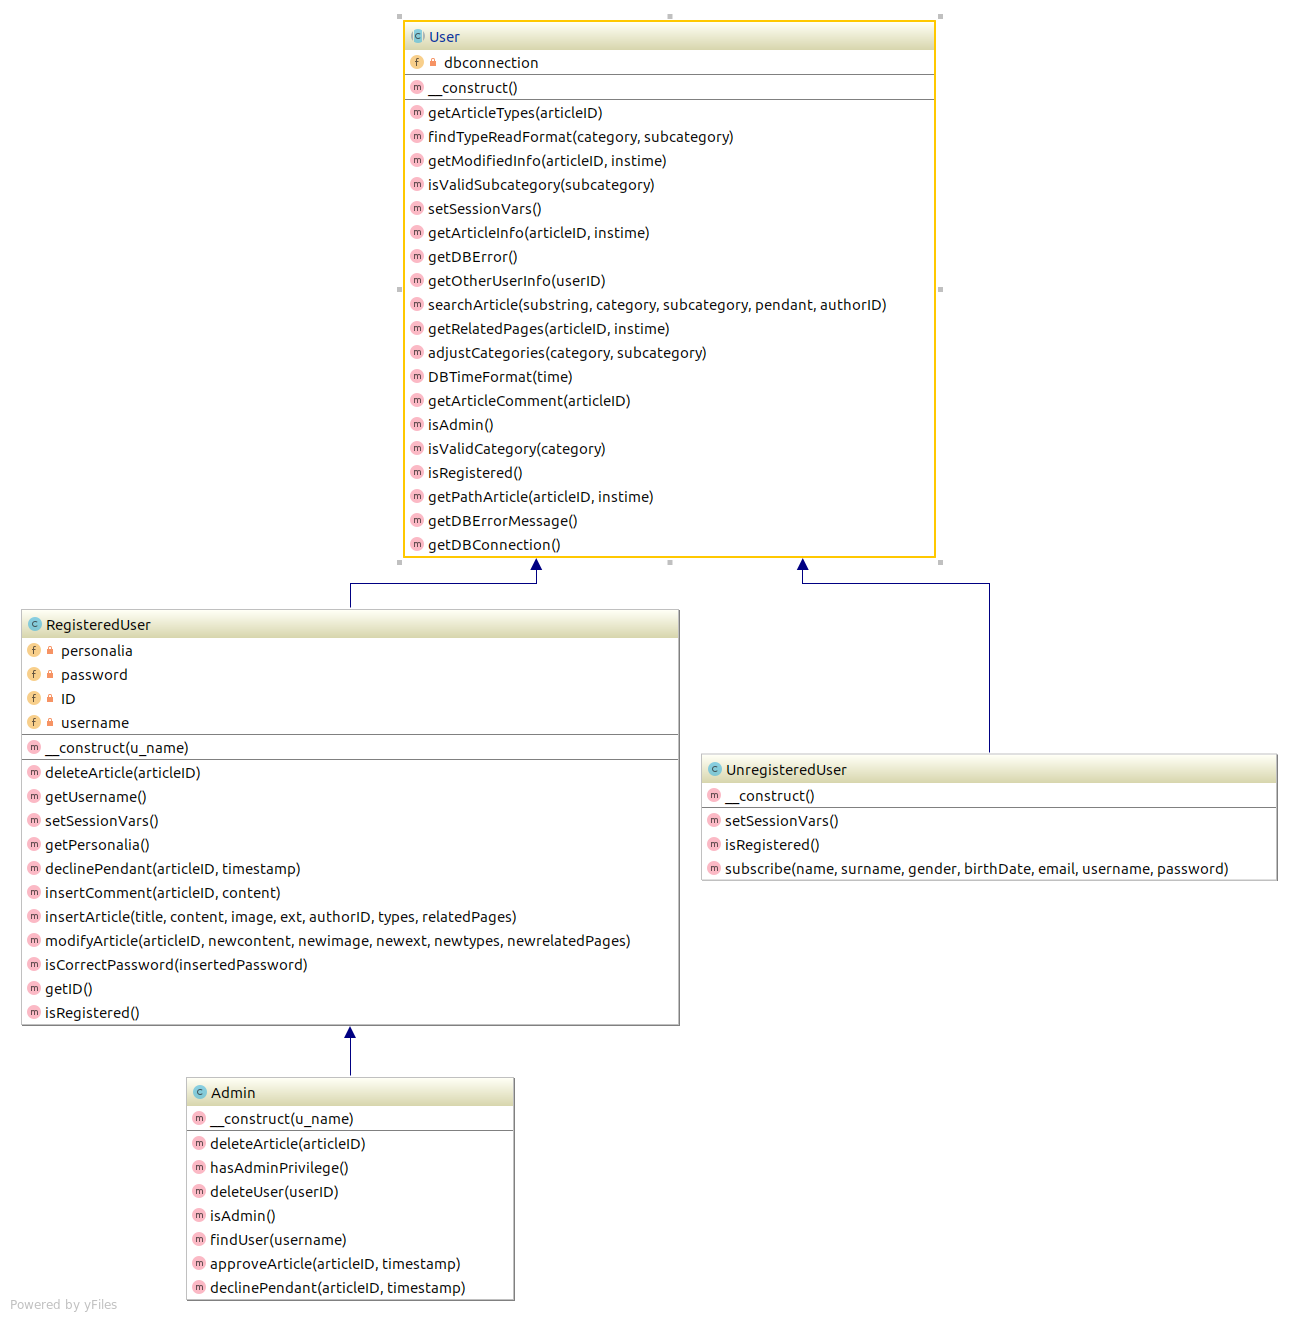
\includegraphics[width=14cm]{img/User.png}
		\caption{Gerarchia utenti}
	\end{center}
\end{figure}

\paragraph{Gerarchia Page} Abbiamo definito una classe che rappresenta una pagina generica. La responsabilità principale di Page e della gerarchia sottostante è quella di gestire la visuale da proporre all'utente. La classe \textit{Page} viene specializzata in tre sottoclassi: \textit{ArticlePage} che gestisce la vista di un articolo, \textit{SearchPage} che gestisce la vista delle pagine con i risultati di ricerca e \textit{FormPage} che gestisce la vista delle pagine con i form.

\subparagraph{Page}
La classe \textit{Page} si occupa della visualizzazione di tutti quegli elementi condivisi da più pagine e di tutte quelle componenti che potrebbero servire in più tipi di pagine.\\
I metodi principali sono:
\begin{itemize}
	\item \texttt{printLogButtons()}: visualizza i bottoni in alto a destra in base alla tipo di utente connesso;
	\item \texttt{printFeedBack()}: si occupa di visualizzare un messaggio di feedback (positivo o negativo).
\end{itemize}

\subparagraph{SearchPage}
La classe \textit{SearchPage} si occupa della visualizzazione delle liste dei risultati delle varie pagine (come ad esempio ricerca.php e listapagine.php), gestendo anche la paginazione. Il campo dati administration viene utilizzato per stabilire un livello di amministrazione della lista. I livelli possibili sono 3:
\begin{enumerate}[start=0, label=\textbf{\arabic*$\rightarrow$}]
	\item \textbf{nessun tipo di amministrazione:} non vengono mostrati bottoni per l'amministrazione;
	\item \textbf{abilita la modifica:} vengono mostrati i bottoni di modifica ed eliminazione;
	\item \textbf{abilita l'approvazione:} vengono mostrati i bottoni di approvazione (se i permessi sono sufficienti) e di eliminazione.
\end{enumerate}
I metodi principali sono:
\begin{itemize}
	\item \texttt{printArticleList()}: permette la stampa di una lista di articoli, in base al privilegio ottenuto dall'utente fornito;
	\item \texttt{printUserList()}: permette la visualizzazione della lista degli utenti;
	\item \texttt{printNavigation()}: si occupa di stampare la navigazione in base agli indici individuati.
\end{itemize}

\subparagraph{ArticlePage}
La classe \textit{ArticlePage} si occupa della visualizzazione delle pagine con gli articoli e della relativa pagina discussione. Per questo motivo, possiede come campo dati una \textit{DiscussionArea}. Permette la stampa delle pagine correlate tramite il metodo \texttt{printRelatedPages()} e quella degli articoli tramite \texttt{printArticleComments()}. Infine, gestisce la stampa della text area in fondo alla discussion area (\texttt{showTextArea()}).

\subparagraph{FormPage}
La classe \textit{FormPage} si occupa di controllare la presenza di errori ed eventualmente mostrarli all'utente. Inoltre, si occupa della visualizzazione dei form in generale.\\
I suoi metodi principali sono:
\begin{itemize}
	\item \texttt{inferRegistrationErrors()}: permette di desumere in base all'array \texttt{\$\_POST} ricevuto in \texttt{registrazione.php} se vi sono stati errori e, nel caso in cui ciò si verifichi, li memorizza nell'array \texttt{\$this->errors};
	\item \texttt{hasErrors()}: in base agli errori contenuti in \texttt{\$this->errors} restituisce \texttt{true} in caso vi siano errori nel form. 
\end{itemize}

\begin{figure}[H]
	\begin{center}
		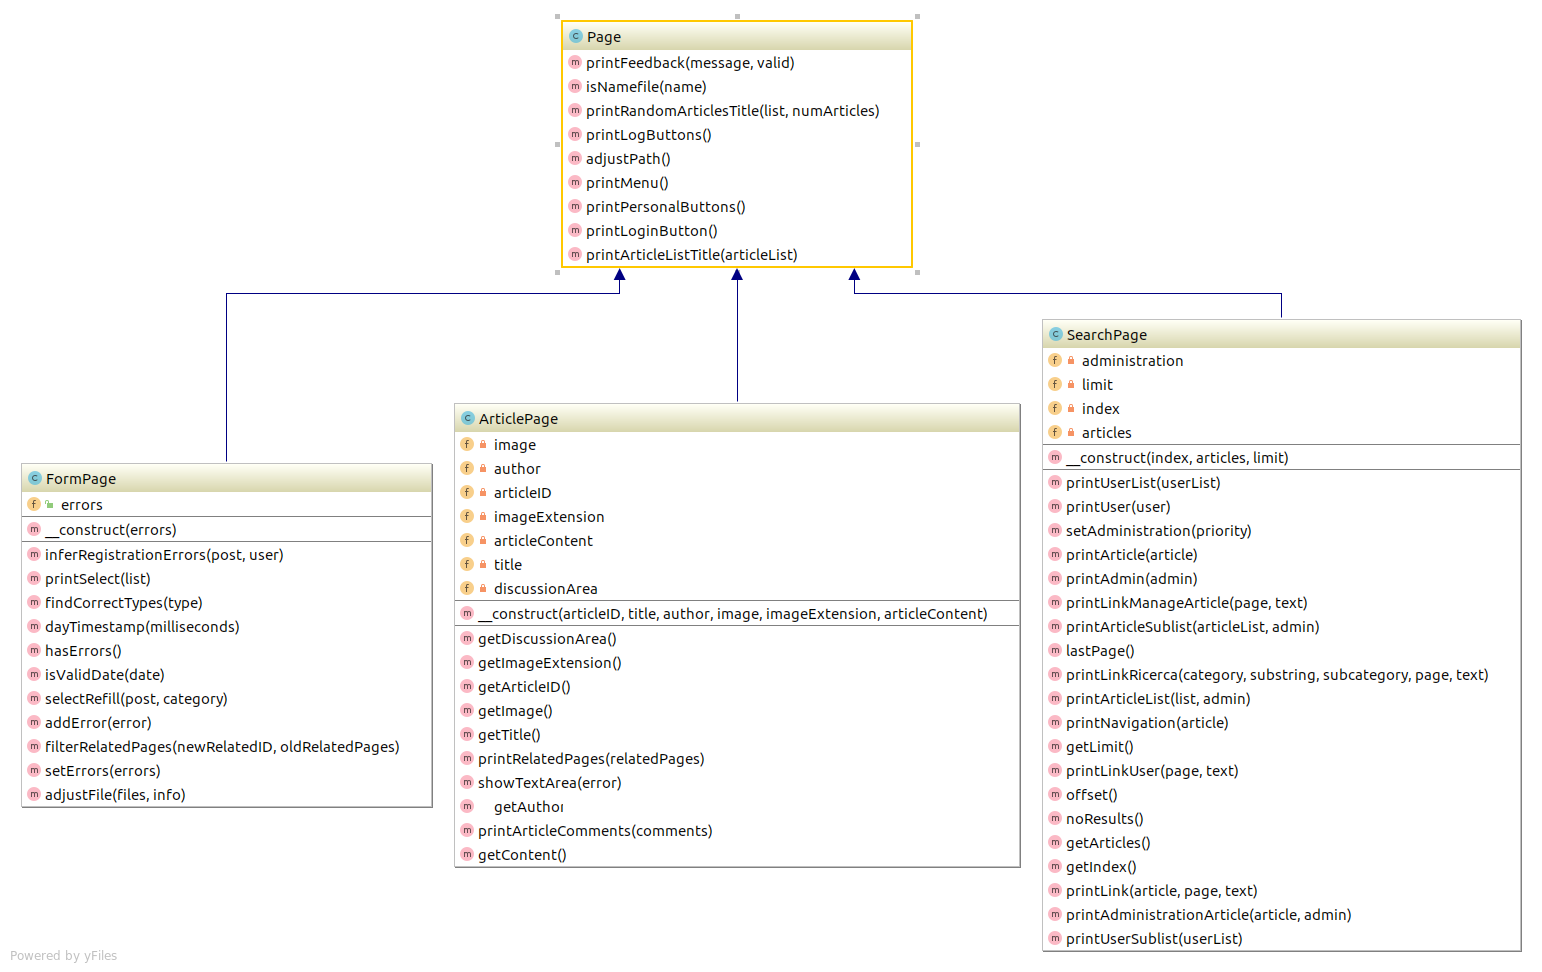
\includegraphics[width=15cm]{img/Page.png}
		\caption{Gerarchia pagine}
	\end{center}
\end{figure}

\paragraph{Discussion Area} Questa classe rappresenta l'area di una pagina in cui compare una discussione, ovvero contiene dei commenti relativi ad un determinato articolo che gli utenti hanno scritto. Questa classe ha una dipendenza verso la classe \textit{Comment}. Questa classe permette l'aggiunta di uno o più commenti, l'eliminazione e la stampa.
\begin{figure}[H]
	\begin{center}
		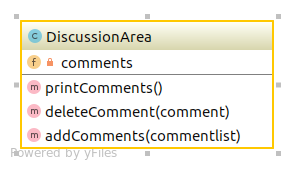
\includegraphics[width=10cm]{img/DiscussionArea.png}
		\caption{Classe Discussion Area}
	\end{center}
\end{figure}

\paragraph{Database Connection} Questa classe rappresenta la connessione al database e permette all'utente di fare delle query al database tramite le funzioni di MySQLi. Permette la visualizzazione degli errori nelle interrogazioni e la possibilità di disconnettersi dal database e collegarsi ad un altro.
\begin{figure}[H]
	\begin{center}
		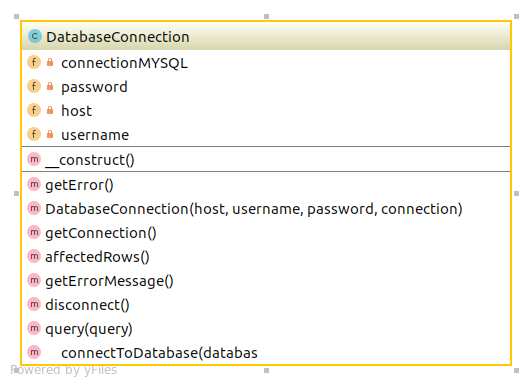
\includegraphics[width=10cm]{img/DatabaseConnection.png}
		\caption{Classe Database Connection}
	\end{center}
\end{figure}

\paragraph{Comment} Questa classe rappresenta un commento fatto da un utente, relativo ad un articolo pubblicato.
\begin{figure}[H]
	\begin{center}
		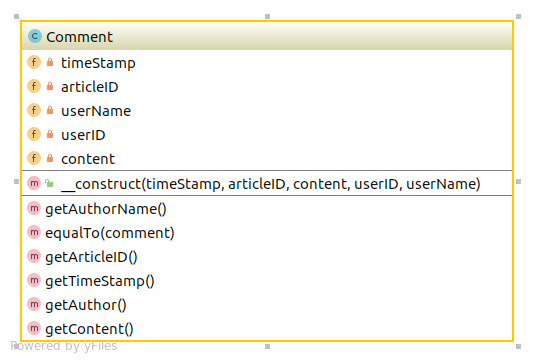
\includegraphics[width=10cm]{img/Comment.png}
		\caption{Classe Comment}
	\end{center}
\end{figure}
\pagebreak
\subsubsection{Sessione}
La sessione viene usata per memorizzare gli ID degli utenti che visitano il sito. In questo modo si può capire la tipologia di utente che sta visitando il sito. Se un utente è non registrato, gli viene asegnato un ID con valore uguale a -1.

\subsubsection{Form} Tutti i tag input vengono sottoposti ad un processo di validazione per garantire un corretto inserimento del dato richiesto. Nel caso un input non superi la validazione, viene mostrato un messaggio di errore senza eliminare il contenuto degli input, cosi che l'utente non debba riscrivere tutti campi nuovamente.
